% http://fachschaft.physik.uni-dortmund.de/images/GlobaltutAP/protokoll.txt
% ========================================
%	Header einbinden
% ========================================

% http://fachschaft.physik.uni-dortmund.de/images/GlobaltutAP/apheader.txt
% ==================================================
%	Festlegung der Dokumentenklasse
% ==================================================


\documentclass[paper=a4, 		% Layout für DinA4
	ngerman				% Deutsche Spracheinstellungen
	]
	{scrartcl} 			% Dokumentklasse für Aufsätze oder z.B. Praktikumsprotokolle

\usepackage{fixltx2e}			% Behebt ein paar Fehler in Latex

% ==================================================
%	Einstellen des Encodings
% ==================================================

\usepackage{ifxetex}
\usepackage{ifluatex} 

\ifxetex
	\usepackage{fontspec}
  	\usepackage{xunicode}
	\usepackage{xltxtra}
    \defaultfontfeatures{Mapping=tex-text} 	% To support LaTeX quoting style
	\setmainfont{Linux Libertine}
=======
    \defaultfontfeatures{Mapping=tex-text} % To support LaTeX quoting style
	\setmainfont{Linux Libertine} % Hier gewünschte Schriftart einfügen
\else
	\ifluatex
		\usepackage{fontspec}		% Falls das nicht funktioniert: \usepackage{luainputenc}
  		\usepackage{xunicode}
  		\defaultfontfeatures{Mapping=tex-text} % To support LaTeX quoting style
		\setmainfont{Linux Libertine} % Hier gewünschte Schriftart einfügen
	\else %pdfTeX
	  \usepackage[utf8]{inputenc}
	  \usepackage[T1]{fontenc}
	 \fi
\fi


% ==================================================
%	Spracheinstellungen
% ==================================================

\usepackage[ngerman]{babel,		% neue deutsche Rechtschreibung
	varioref}			% Bei Referenzen wird der Name des Objektes vor die Refernznummer geschrieben: z.B. \ref{bsp} liefert Seite 1

% ==================================================
%	Referenzen und Links
% ==================================================

\usepackage{hyperref}			% Verlinkungen innerhalb und außerhalb des PDF-Dokuments
\usepackage{url}			% Formattiert URLs, so dass sie sich z.B. besser vom Text abheben
\urlstyle{tt}				% TrueType-Schrift für URLs		



% ==================================================
%	Bibliograhphie
% ==================================================
%Zwei verschiedene Möglichkeiten Bibliographien einzubinden:

%	Möglichkeit 1:
% ========================
	\usepackage[numbers]{natbib}	%Paket für Bibliograhien

	%Bibtex: Nachnamen in Kapitälchen
	%\renewcommand*{\mkbibnamelast}[1]{\textsc{#1}}
	\newcommand*{\mkbibnamelast}[1]{\textsc{#1}}

	% Makros für Anhang + Referenzen
	\newcommand{\anhang}{
		\clearpage		% Anhang auf eine extra Seite packen
		\setcounter{page}{0}	
		\pagenumbering{Roman}	% Anhang wird in römischen Seitenzahlen numeriert
		\appendix		% Kapitelnummerierung in Großbuchstaben statt Zahlen.
	}

	\newcommand{\referenzen}{
		\bibliographystyle{alphadin} 			% Alphabetisch sortiert im DIN-Format
		\addcontentsline{toc}{section}{Referenzen}
		\phantomsection					% Referenzen ins Inhaltsverzeichnis
		\renewcommand{\refname}{\section*{Referenzen}\vspace*{-1em}} % Benennt das Kapitel um
		\bibliography{../include/Bibliographie.bib} 	% Die BibTeX-Datei einbinden
	}
%Zu Verwenden mit \bibliography{BIBDATEI}
% ========================
%	Möglichkeit 2:
% ========================
	%\usepackage{csquotes}				%Wird für Biblatex benötigt
	%\usepackage[style=alphabetic]{biblatex}	%Paket für Bibliograhphien mit Biblatex
%Zu Verwenden mit \bibliography{BIBDATEI} und \printbibliography oder \printbibliography[heading=bibintoc] (falls ein Inhaltsverzeichns verwendet wird)
% ==================================================



% ==================================================
%	Grafiken, Abbildungen und Tabellen
% ==================================================

\usepackage{graphicx}                   % zum Einbinden von Grafiken
\usepackage{xcolor}			% Für die Verwendung von Farben
\usepackage[font=small,			% kleine Schrift für Bildunterschriften
	labelfont=bf			% Fettgedruckte Bildunterschriften
	]
	{caption}			% Für Bildunterschriften

\usepackage{subcaption}			% Für mehrere Objekte nebeneinander mit eigenen Bildunterschriften

\usepackage{tabularx}			% Erweiterte Befehle für Tabellen
\usepackage{booktabs}			% Für professionele Tabellen, siehe Manual
\usepackage{longtable}			% Für Tabellen, die nicht mehr auf eine Seite passen.

\usepackage{rotating}			% Zum Verdrehen von Objekten. Nur mäßig verwenden.

%\graphicspath{{figs/}{bilder/}}	% Bildverzeichnisse MUSS ÜBERPRÜFT WERDEN!!!

% ==================================================
%	Mathematikumgebungen und Einheiten
% ==================================================

\usepackage{amsmath}			% Paket für mathematische Umgebungen und Funktionen
\usepackage{amsfonts}			% Zusätzliche Mathematische Schriftarten
\usepackage{amssymb}			% Zusätzliche Mathematische Symbole
%\usepackage{amscd}			% Zum Setzen Kommutativer Diagramme
\usepackage{amstext}			% Textsatz in der Matheumgebung
\usepackage{upgreek}			% Aufrechte griechische Buchstaben


% Diagramme mit tikz und Gnuplot zeichnen
%	\usepackage{tikz}
%	\usepackage{tikz-qtree}
%	\usepackage{gnuplot-lua-tikz}

% ==================================================
% SIUnitX: Einheiten werden vollautomatisch gesetzt
% ==================================================
\usepackage[
    separate-uncertainty = true, 		% Stellt den Fehler separat dar: Siehe SIUnitX-Manual
    mode 			= text, 	% Stellt Einheiten (Kelvin etc.) Nichtkursiv dar
    quotient-mode	= 	fraction,	% Bruchstriche nutzen
    repeatunits           = false, 
    range-phrase          = {\,bis\,},  
]{siunitx}
\sisetup{
	per-mode = fraction, 			% Bruchstriche nutzen
	output-decimal-marker = {,}, 		% Setzt das Dezimaltrennzeichen als Komma
	multi-part-units = brackets,
	exponent-product = \cdot,
}

\addto\extrasgerman{\sisetup{locale = DE}}	% "Deutsche" Einheiten
\usepackage{cancel}				% Kürzen von Einheiten in SIUnitX ermöglichen


% ==================================================
%	Sonstiges
% ==================================================

%\usepackage[official]{eurosym}			% offizielles Eurosymbol

% ==================================================
%	Seitenlayout
% ==================================================

% Kein Einrücken der Absätze (Einrücken = Null)
	\setlength{\parindent}{0pt}             % kein Einrücken der ersten Zeile in einem neuen Absatz

% Vermeidung von "Schusterjungen"
	\clubpenalty = 3000			% Höchstwert 10000, dann dürfen theoretisch keine Schusterjungen mehr auftreten.
% Vermeidkung von "Hurenkindern"
	\widowpenalty = 3000			% Höchstwert 10000, dann dürfen theoretisch keine Hurenkinder mehr auftreten.
	\displaywidowpenalty = 3000		% Es werden beide Einstellungen benötigt.

% Seitenlayout ändern mit Fancy
	\usepackage{fancyhdr}			% Paket zum bequemeren Verändern des Seitenlayouts

	% Tabellen ändern:
		\renewcommand{\thetable}{\arabic{section}.\arabic{table}} % figures bekommen die richtige Nummerierung: x.y
		\makeatletter \@addtoreset{table}{section} \makeatother      % nach jeder section wird neu gezählt

	% Kapitelüberschriften in der Kopfzeile:
		\renewcommand*{\sectionmark}[1]{\markboth{}{\thesection\ #1}}
		%\renewcommand*{\subsectionmark}[1]{\markboth{}{\thesubsection\ #1}}
		\renewcommand*{\subsectionmark}[1]{\markboth{}{}} % keine Unterüberschriften in der Kopfzeile
		\renewcommand{\plainheadrulewidth}{0.4pt}
	
	% Seitennummern rechts in der Kopfzeile:
		\lhead[\fancyplain{\thepage}{\thepage}]{\fancyplain{}{\rightmark}}
		\rhead[\fancyplain{}{\leftmark}]{\fancyplain{\thepage}{\thepage}}
	
	%Fußzeilen bleiben leer
		\lfoot{}
		\cfoot{}
		\rfoot{}
		
%Eigenes
\usepackage[section]{placeins}
\renewcommand*\rmdefault{iwona}\normalfont\upshape

% ========================================
%	Angaben für das Titelblatt
% ========================================

\title{Versuch 351 - Fourier-Analyse und Synthese\\				% Titel des Versuchs 
\large TU Dortmund, Fakultät Physik\\ 
\normalsize Anfänger-Praktikum}

% \author{Marc Posorske\\			% Name Praktikumspartner A
% {\small \href{marc.posorske@tu-dortmund.de}{marc.posorske@tu-dortmund.de}}	% Erzeugt interaktiven einen Link
% \and						% um einen weiteren Author hinzuzfügen
% Fabian Lehmann\\					% Name Praktikumspartner B
% {\small \href{fabian.lehmann@tu-dortmund.de}{fabian.lehmann@tu-dortmund.de}}		% Erzeugt interaktiven einen Link
% }

\author{Fabian Lehmann\\					% Name Praktikumspartner B
{\small \href{fabian.lehmann@tu-dortmund.de}{fabian.lehmann@tu-dortmund.de}}		% Erzeugt interaktiven einen Link
}

\date{13. Dezember 2012}%21.Dezember 2012}				% Das Datum der Versuchsdurchführung

% ========================================
%	Das Dokument beginnt
% ========================================

\begin{document}

% ========================================
%	Titelblatt erzeugen
% ========================================

\maketitle					% Jetzt wird die Titelseite erzeugt
\thispagestyle{empty} 				% Weder Kopfzeile noch Fußzeile

% ========================================
%	Der Vorspann
% ========================================

%\newpage					% Wenn Verzeichnisse auf einer neuen Seite beginnen sollen
%\pagestyle{empty}				% Weder Kopf- noch Fußzeile für Verzeichnisse

\tableofcontents

%\newpage					% eine neue Seite
%\thispagestyle{empty}				% Weder Kopf- noch Fußzeile für Verzeichnisse
%\listoffigures					% Abbildungsverzeichnis

%\newpage					% eine neue Seite
%\thispagestyle{empty}				% Weder Kopf- noch Fußzeile für Verzeichnisse
%\listoftables					% Tabellenverzeichnis
\newpage					% eine neue Seite


% ========================================
%	Kapitel
% ========================================

%\section{Einleitung}				% Bei Bedarf
%	%
%

\section{Theorie}
	%picfouana
%eqfou1,eqfout2,eqfoua,eqfoub
\subsection{Einführung}
Die Fourier-Analyse und Synthese mit der Fourier-Transformation beschreiben Verfahren, die 
Funktionen durch unendliche Reihen, beziehungsweise Integrale über einen unendlichen Bereich,
annähern.\\
\subsection{Fourier-Analyse} 
	\begin{figure}[h]
		\begin{center}
		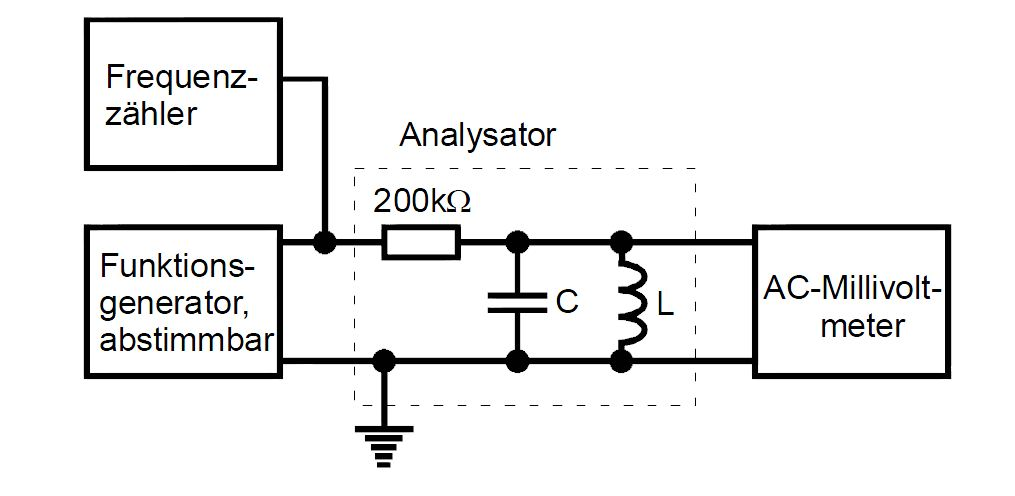
\includegraphics[scale=0.4]{picfouana.jpg}
		\caption{Schaltung zur Fourier-Analyse [1]}
		\label{picfouana}
		\end{center}	
	\end{figure}
Periodischen Funktionen $f$ mit der Periodendauer $T$ lassen sich durch Cosinus- und Sinusfunktionen
beschreiben (Gl. \ref{eqfou1}, \cite{anleitung}). Gleichheit in Gleichung (\ref{eqfou1}) gilt bei den meisten physikalischen Prozessen.
\begin{align}
f(t) &\sim \frac{a_0}{2} + \sum_{n=1}^{\infty} (a_n \text{ } cos(n \text{ } \frac{2 \pi}{T} t) + b_n \text{ } sin(n \frac{2 \pi}{T}) t) \label{eqfou1} \\
a_n &= \frac{2}{T} \int_0^T f(t) cos(n \frac{2 \pi}{T} t) \text{ dt} \text{ , } n=1,2, \ldots \label{eqfoua}\\
b_n &= \frac{2}{T} \int_0^T f(t) sin(n \frac{2 \pi}{T} t) \text{ dt} \text{ , } n=1,2, \ldots \label{eqfoub}
\end{align}
Die Fourier-Analyse beschreibt das Ermitteln der Vorfaktoren, beziehungsweise der Amplituden $a_n$ und $b_n$ für bekannte Funktionen.
Dabei kann man sich zunutze machen, dass bei geraden Funktionen $f$ alle $b_n=0$ werden und bei
ungeraden Funktionen alle $a_n$ verschwinden. Die Darstellung der Amplituden in Abhängigkeit zu von der zugehörigen Frequenz $n/T$
heißt Frequenzspektrum. Ein solches lässt sich beispielsweise mit einer Schaltung wie in Abbildung (\ref{picfouana})
bestimmen, welche auf der Proportionalität zwischen Resonanzspannung und Amplitude der Oberwellen beruht.
\subsection{Fourier-Synthese}
Im Gegensatz dazu wird bei der Fourier-Synthese eine Funktion aus bekannten Koeffizienten zusammengesetzt.
Durch schrittweises Hinzufügen der einzelnen Summanden wird die Funktion angenähert. Bei der
praktischen Umsetzung können Lissajous-Figuren, Kurven, die bei einer Schwingungsüberlagerung entstehen, helfen, 
die Phase der einzelnen Komponenten zu kalibrieren.
\subsection{Gibbsches Phänomen}
Das Gibbsche Phänomen tritt auf, wenn die Funktion $f(t)$ Unstetigkeiten aufweist. An den Stellen
der Unstetigkeit tritt immer ein endlicher Über-, beziehungsweise Unterschwung auf, da diese Stellen
nicht approximiert werden können.
\subsection{Fourier-Transformation}
Mit der Fourier-Transformation lässt sich das gesamte Frequenzspektrum, unabhängig einer
möglichen Periodizität der Funktion, bestimmen. Ähnlich zu Gleichung (\ref{eqfou1}) lässt sich auch die 
Fourier-Transformation beschreiben.
\begin{align}
f(t)&=\frac{1}{2 \pi} \int_{-\infty}^{\infty} g(\nu) e^{-i \nu t} \text{ d}\nu \\
g(\nu)&=\int_{-\infty}^{\infty} f(t) e^{i \nu t} \text{ dt} \label{eqfout2}
\end{align}

	\FloatBarrier
\section{Durchführung}
	%
%
\subsection{Fourier-Synthese}
Zuerst wird mit einem Oszilloskop der Oberwellensynthesizer auf die richtige 
Phasenlage kalibriert. Dazu wird die Grundschwingung auf den X-Eingang und die 
einzustellende Schwingung auf den Y-Eingang gelegt. Dann wird die dabei enstehende
Lissajous-Figur soweit durch ver�ndern der Phase ver�ndert, bis eine einzelne Kurve
zu sehen ist. Dann kann durch Phasenspr�nge von $90\circ$ oder $180\circ$ die Phase
zu den Oberwellen passend eingestellt werden.\\
Jetzt werden die vorher berechneten Amplituden der Fourierreihenkomponenten mit dem
Synthesizer angepasst und dann schrittweise unter Phasenlagen�berpr�fung addiert und
auf einem Oszilloskop ausgegeben. Das ganze wird je f�r eine Dreieck-, eine S�gezahn- und
eine Rechteckspannung durchgef�hrt. 
\subsection{Fourier-Analyse}
Ein passend eingestellter Funktionengenerator wird an ein Oszilloskop mit eingebautem Rechner
angeschlossen, welcher eine Fourieranalyse (vgl. Gl. \ref{eqfout2}) durchf�hrt und auf dem Bildschirm
ausgibt. Dann werden mit dem Cursor die Amplituden der einzelnen Schwingungsbestandteile abgelesen.
	\FloatBarrier
\section{Auswertung}
	%picfdrei,picfrecht,picfsage,picfsr,picfsd,picfss,picfar,picfad,picfas
%tabfsr,tabfsd,tabfss,tabfar,tabfad,tabfas
%subsec:rechnen
\subsection{Berechnung der Fourier-Koeffizienten} \label{subsec:rechnen}
	\begin{figure}[h]
		\begin{center}
		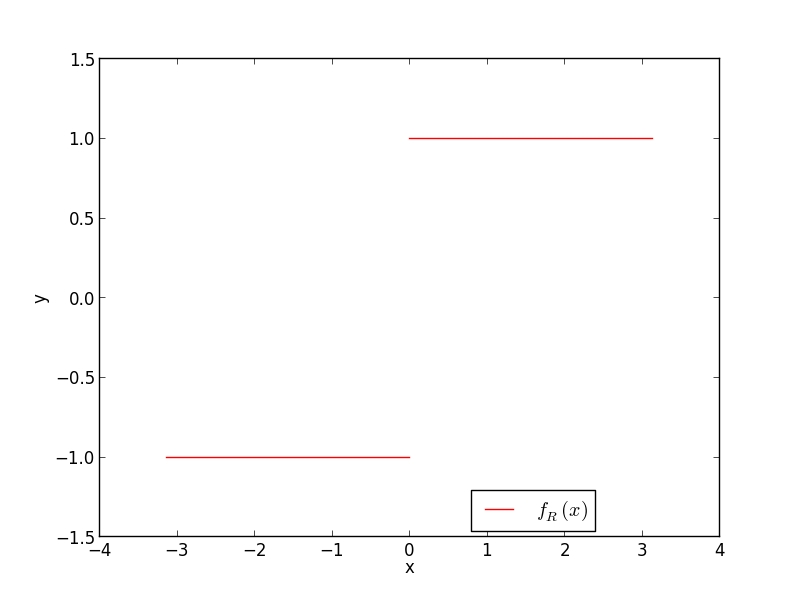
\includegraphics[scale=0.42]{picfrecht.jpg}
		\caption{Periodisch fortzusetzende Funktion $f_R$}
		\label{picfrecht}
		\end{center}	
	\end{figure} 	\begin{figure}[h]
		\begin{center}
		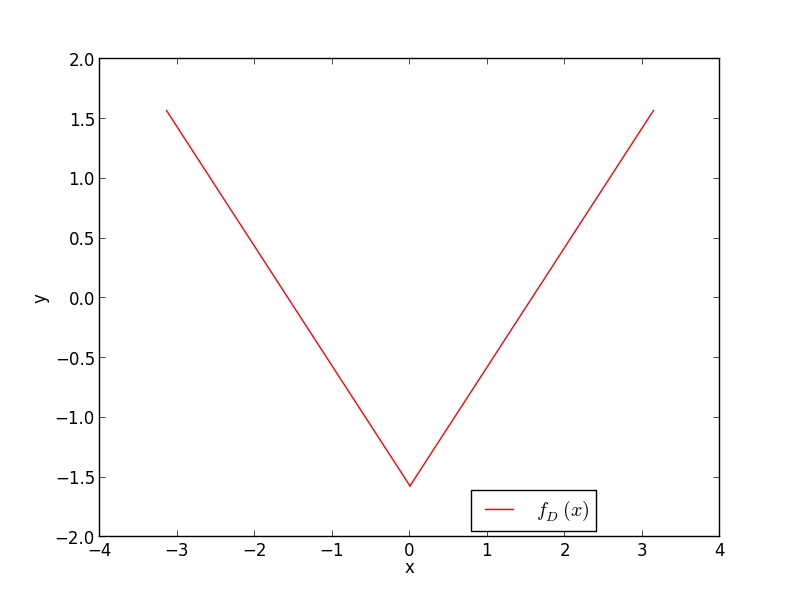
\includegraphics[scale=0.42]{picfdrei.jpg}
		\caption{Periodisch fortzusetzende Funktion $f_D$}
		\label{picfdrei}
		\end{center}	
	\end{figure} 	\begin{figure}[h]
		\begin{center}
		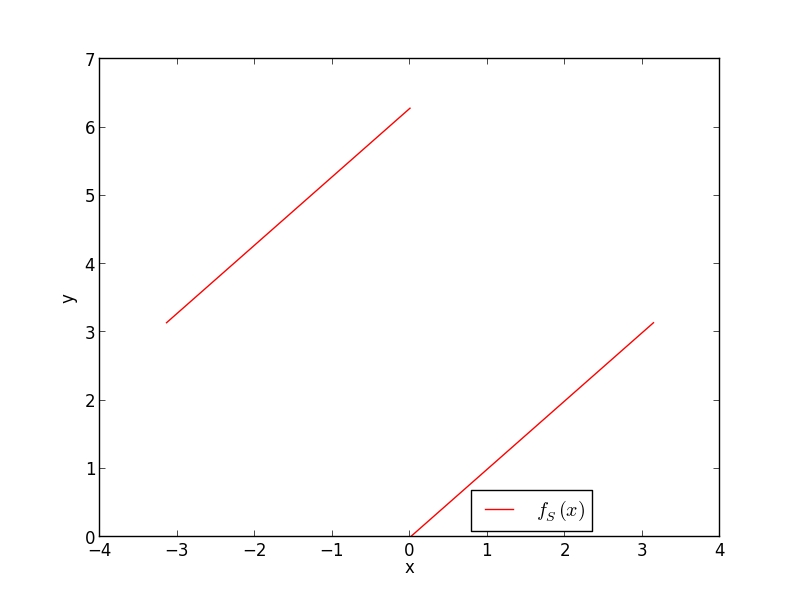
\includegraphics[scale=0.42]{picfsage.jpg}
		\caption{Periodisch fortzusetzende Funktion $f_S$}
		\label{picfsage}
		\end{center}	
	\end{figure}
Die Koeffizienten der einzelnen periodischen Funktionen berechnen sich nach den 
Gleichungen (\ref{eqfoua}) und (\ref{eqfoub}). Dabei wurde die Rechteckfunktion 
$f_R$, Abbildung (\ref{picfrecht}), als ungerade Funktion gewählt, für alle $i$ ist $a_i=0$.
Die Dreieckfunktion $f_D$, Abbildung (\ref{picfdrei}), und die Sägezahnfunktion $f_S$,
Abbildung (\ref{picfsage}), sind als gerade Funktionen definiert worden, für alle $i$ gilt
also  $b_i=0$.
\begin{align}
\text{Es gilt für die Funktionen der Definitionsbereich }&\pi \ge x > -\pi \text{ mit einer periodischen} \nonumber \\
\text{Fortsetzung von }T=2\pi \text{ .}\nonumber \\
f_R(x)&=\frac{\left| x \right|}{x}\\
f_D(x)&=\left| x \right| - \frac{\pi}{2}\\
f_S(x)&=\begin{cases}
  x + 2 \pi,  & -\pi \le x < 0\\
  x, & 0 \le x < \pi
\end{cases}\\
\text{Es ergeben sich die folgenden Fourierkoeffizienten }&\text{mit $N=1,2, \ldots$.} \nonumber \\
f_R: a_0&=0,\text{ }a_n=0, \\
b_n&=\begin{cases}
	\frac{4}{n\pi}, & n \text{ ungerade}\\
	0, & n \text{ gerade}
\end{cases}\\
f_D: a_0&=0, \text{ }b_n=0,\\
a_n&=\begin{cases}
	-\frac{4}{n^2\pi}, & n \text{ ungerade}\\
	0, & n \text{ gerade}
\end{cases}\\
f_S: a_0&=\pi, \text{ }a_n=0, \text{ }b_n=-\frac{2}{n}
\end{align}
\subsection{Fourier-Synthese}
\begin{table}[h]
	\begin{center}
		\begin{tabular}{cc}
			n&b$_\text{n}$/mV \\ \hline
			1&585,90\\
			2&0,00\\
			3&195,30\\
			4&0,00\\
			5&117,18\\
			6&0,00\\
			7&83,70\\
			8&0,00\\
			9&65,10
		\end{tabular}
		\caption{Amplituden der Fourier-Koeffizienten bei Synthese der Rechteckspannung (a$_\text{0}=\text{a}_\text{n}=0\text{ mV}$)}
		\label{tabfsr}
	\end{center}
\end{table} \begin{table}[h]
	\begin{center}
		\begin{tabular}{cc}
			n&a$_\text{n}$/mV \\ \hline
			1&585,90\\
			2&0,00\\
			3&65,10\\
			4&0,00\\
			5&23,44\\
			6&0,00\\
			7&11,96\\
			8&0,00\\
			9&7,23
		\end{tabular}
		\caption{Amplituden der Fourier-Koeffizienten bei Synthese der Dreieckspannung (a$_\text{0}=\text{b}_\text{n}=0\text{ mV}$)}
		\label{tabfsd}
	\end{center}
\end{table} \begin{table}[h]
	\begin{center}
		\begin{tabular}{cc}
			n&b$_\text{n}$/mV \\ \hline
			1&585,90\\
			2&292,90\\
			3&195,30\\
			4&146,48\\
			5&117,18\\
			6&97,65\\
			7&83,70\\
			8&73,24\\
			9&65,10
		\end{tabular}
		\caption{Amplituden der Fourier-Koeffizienten bei Synthese der Sägezahnspannung (a$_\text{0}=\text{a}_\text{n}=0\text{ mV}$)}
		\label{tabfss}
	\end{center}
\end{table} 	\begin{figure}[h]
		\begin{center}
		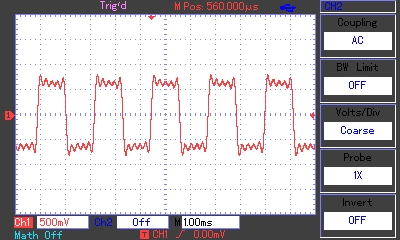
\includegraphics[scale=1.0]{picfsr.jpg}
		\caption{Fouriersynthese der Rechteckspannung}
		\label{picfsr}
		\end{center}	
	\end{figure} 	\begin{figure}[h]
		\begin{center}
		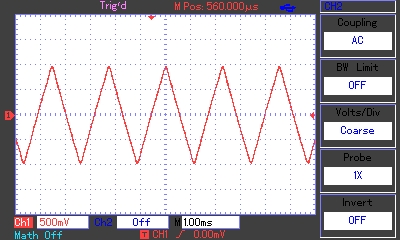
\includegraphics[scale=1.0]{picfsd.jpg}
		\caption{Fouriersynthese der Dreieckspannung}
		\label{picfsd}
		\end{center}	
	\end{figure} 	\begin{figure}[h]
		\begin{center}
		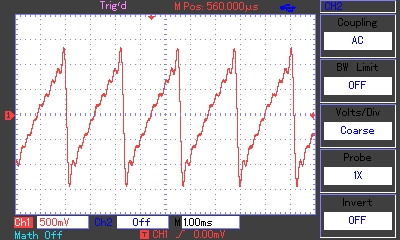
\includegraphics[scale=1.0]{picfss.jpg}
		\caption{Fourier-Synthese der Sägezahnspannung}
		\label{picfss}
		\end{center}	
	\end{figure}
Aus den Koeffizientengleichungen aus \ref{subsec:rechnen} ergeben sich die einzustellenden Amplituden
des Oberwellengenerators (Tab. \ref{tabfsr} - \ref{tabfss}). Nach der Aufsummierung der Oberwellen
ergeben sich die Graphen \ref{picfsr} bis \ref{picfss} auf dem Oszilloskop.
\FloatBarrier
\subsection{Fourier-Analyse}
\begin{table}[h]
	\begin{center}
		\begin{tabular}{cccc}
			n&b$_\text{n,mess}$/mV & b$_\text{n,theorie}$/mV & $\Delta \text{a}_\text{n}$\\ \hline
			1&7320&7320,00&0,0\%\\
			2&0&0,00&0,0\%\\
			3&2960&2440,00&21,3\%\\
			4&0&0,00&0,0\%\\
			5&1460&1464,00&0,3\%\\
			6&0&0,00&0,0\%\\
			7&1010&1045,71&3,4\%\\
			8&0&0,00&0,0\%\\
			9&952&813,33&17,0\%
		\end{tabular}
		\caption{Amplituden der Fourier-Koeffizienten bei Analyse der Rechteckspannung (a$_\text{0}=\text{a}_\text{n}=0\text{ mV}$)}
		\label{tabfar}
	\end{center}
\end{table} \begin{table}[h]
	\begin{center}
		\begin{tabular}{cccc}
			n&a$_\text{n,mess}$/mV & a$_\text{n,theorie}$/mV & $\Delta \text{a}_\text{n}$\\ \hline
			1&4760,0&4760,00&0,0\%\\
			2&0,0&0,00&0,0\%\\
			3&636,0&528,89&20,3\%\\
			4&0,0&0,00&0,0\%\\
			5&162,0&190,40&14,9\%\\
			6&0,0&0,00&0,0\%\\
			7&99,2&97,14&2,1\%\\
			8&0,0&0,00&0,0\%\\
			9&61,2&58,77&4,1\%
		\end{tabular}
		\caption{Amplituden der Fourier-Koeffizienten bei Analyse der Dreieckspannung (a$_\text{0}=\text{b}_\text{n}=0\text{ mV}$)}
		\label{tabfad}
	\end{center}
\end{table} \begin{table}[h]
	\begin{center}
		\begin{tabular}{cccc}
			n&b$_\text{n,mess}$/mV & b$_\text{n,theorie}$/mV & $\Delta \text{a}_\text{n}$\\ \hline
			1&3680&3680,00&0,0\%\\
			2&1800&1840,00&2,2\%\\
			3&1460&1226,67&19,0\%\\
			4&920&920,00&0,0\%\\
			5&716&736,00&2,7\%\\
			6&700&613,33&14,1\%\\
			7&500&525,71&4,9\%\\
			8&464&460,00&0,9\%\\
			9&464&408,89&13,5\%
		\end{tabular}
		\caption{Amplituden der Fourier-Koeffizienten bei Analyse der Sägezahnspannung (a$_\text{0}=\text{a}_\text{n}=0\text{ mV}$)}
		\label{tabfas}
	\end{center}
\end{table} 	\begin{figure}[h]
		\begin{center}
		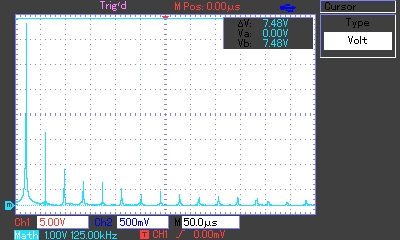
\includegraphics[scale=1.0]{picfar.jpg}
		\caption{Fourieranalyse der Rechteckspannung}
		\label{picfar}
		\end{center}	
	\end{figure} 	\begin{figure}[h]
		\begin{center}
		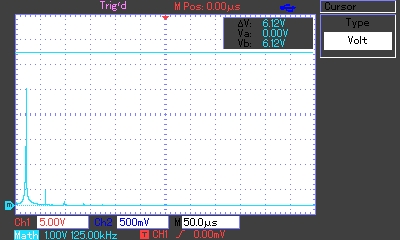
\includegraphics[scale=1.0]{picfad.jpg}
		\caption{Fourieranalyse der Dreieckspannung}
		\label{picfad}
		\end{center}	
	\end{figure} 	\begin{figure}[h]
		\begin{center}
		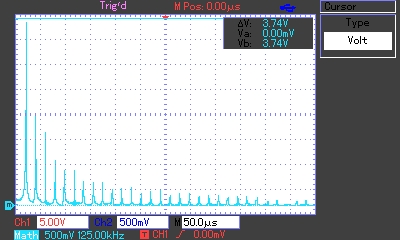
\includegraphics[scale=1.0]{picfas.jpg}
		\caption{Fourieranalyse der Sägezahnspannung}
		\label{picfas}
		\end{center}	
	\end{figure}
Die abgelesenen Amplituden in den Tabellen \ref{tabfar} bis \ref{tabfas} ergeben sich aus den Graphen
\ref{picfar} bis \ref{picfas} des Oszilloskops. Die Theoriewerte ergeben sich dabei aus der Normierung
des ersten Messwertes und der darauf aufbauenden Berechnung gemäß Gleichungen (\ref{eqfoua}) und (\ref{eqfoub}). 

	\FloatBarrier
\section{Diskussion}
	%
%

	\FloatBarrier
% ========================================
%	Literaturverzeichnis
% ========================================

\bibliographystyle{plainnat}			% Bibliographie-Style auswählen
\bibliography{lit}			% Literaturverzeichnis

% ========================================
%	Das Dokument endent
% ========================================
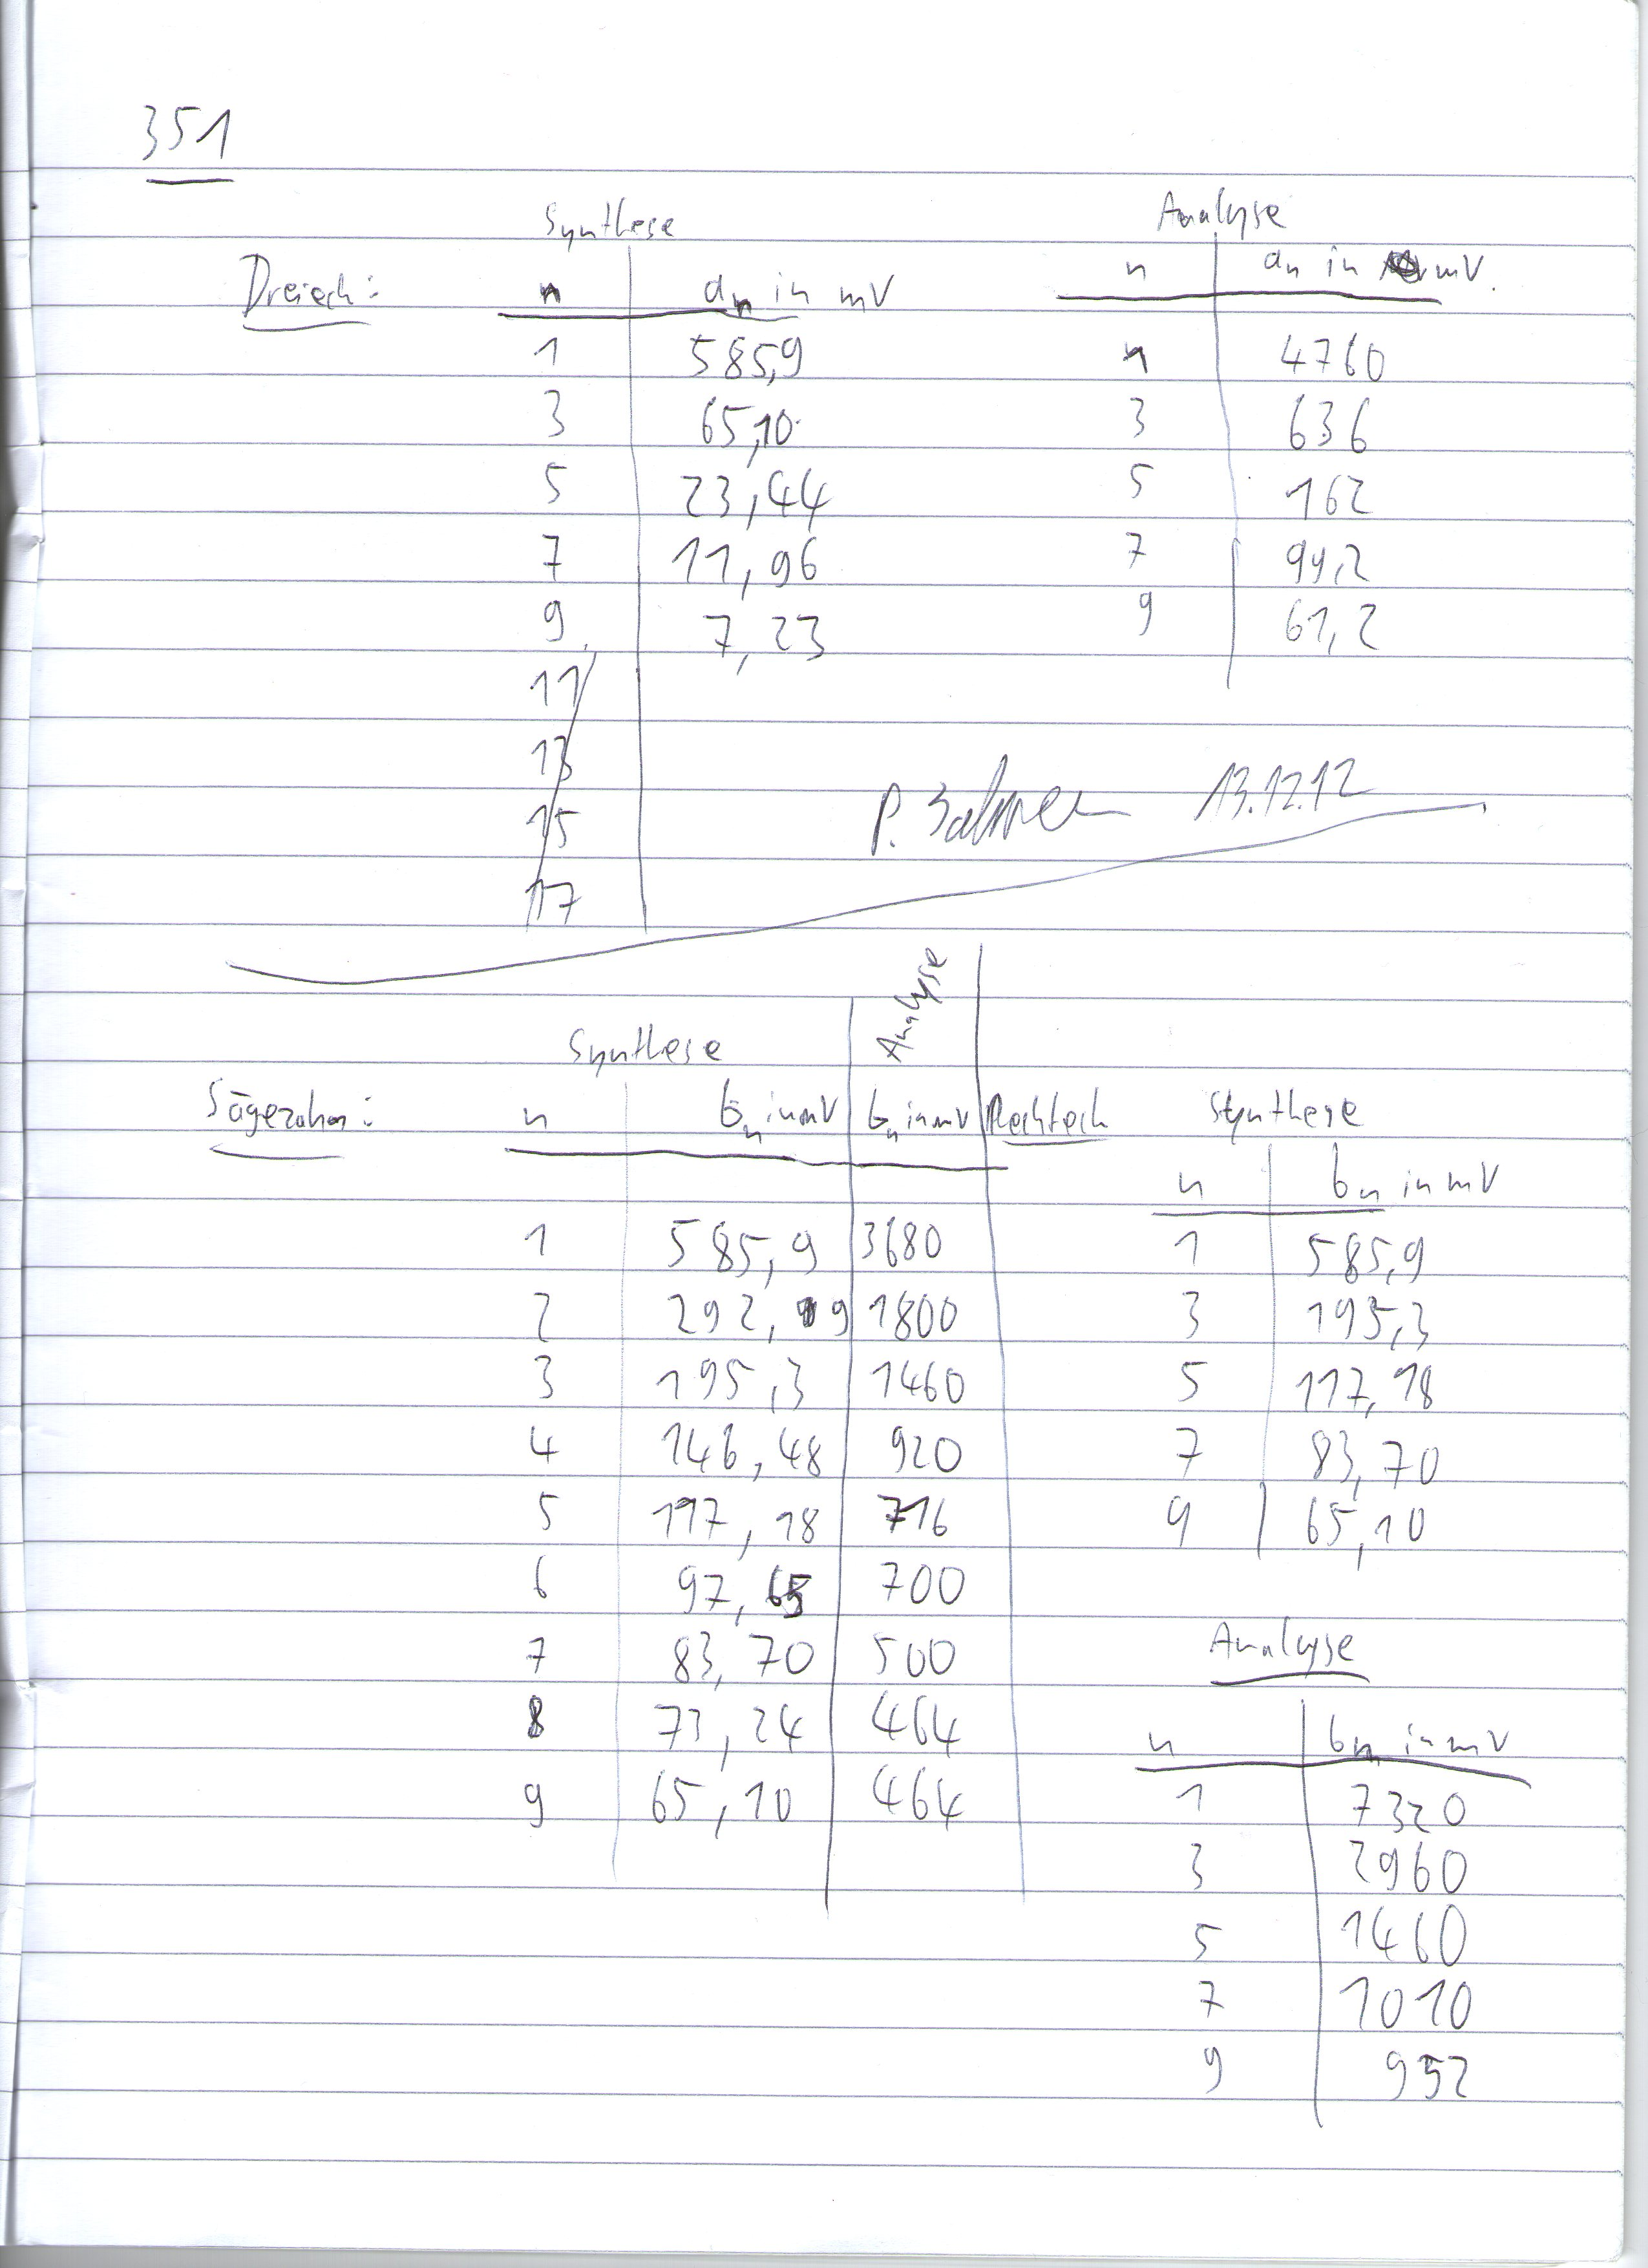
\includegraphics[scale=0.75]{img015.jpg}
\end{document}